\begin{figure*}
  \centering
  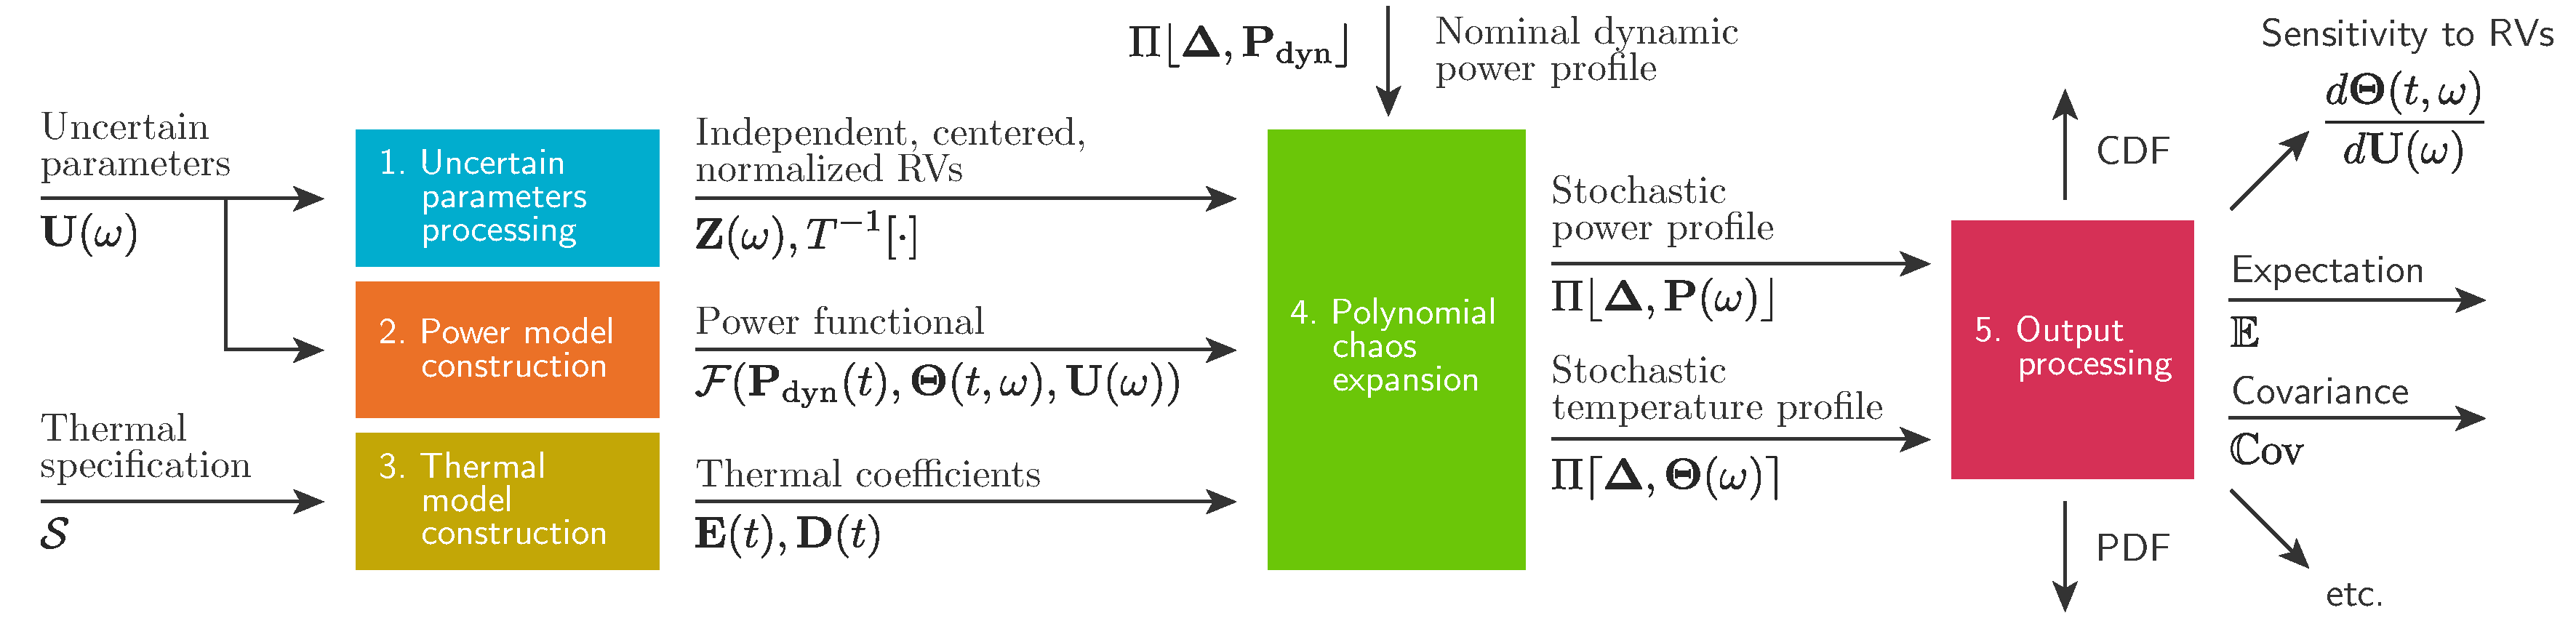
\includegraphics[width=0.9\textwidth]{include/assets/algorithm.pdf}
  \vspace{-0.7em}
  \caption{The structure of the proposed framework.}
  \flabel{algorithm}
  \vspace{-1.6em}
\end{figure*}

In a nutshell, the goal stated in \sref{problem-formulation} is achieved as follows. We begin with the commonly found formalism of constructing a thermal model given a thermal specification $\system$. Due to the complexity of the underlying physical phenomenon---that is, heat trasfer within a multiprocessor system---such a model is expensive from the computational perspective; this fact makes the straightforward UQ based on MC simulations prohibited and often infiasible. Instead of working directly with the obtained model, we construct a surrogate model, or a meta model, using the theory of polynomial chaos (PC) expansions. Such a representation is essentially light, \ie, the effords needed to obtain power and temperature traces, given an assignment of the uncertain parameters, are negligible compared to those needed for the initial problem formulation. Now, the surrogate model can undergo the same sampling that one might adopt from the very beginning, but this time the procedure is undertaken in a much more efficient manner. Therefore, such quantities as \cdfs\ and \pdfs\ can be trivially estimated. Moreover, the representations, which we compute, provide analytical formulae for probabilistic moments, \ie, the expected value, variance, \etc\ are readily available without any sampling.

The major steps of our technique are depicted in \fref{algorithm} and are ourlined below whereas detailed discussions are given in the following five subsections, \sref{uncertain-parameters}--\sref{output-processing}.

\step{1}{Uncertain Parameters (\sref{uncertain-parameters}).} PC, employed in this paper to perform UQ, operate on a finite set of independent \rvs. The uncertain parameters $\vU(\o)$ might not satisfy this requirement and, therefore, should be preprocessed first; the corresponding finite, independent set is denoted by $\vZ(\o)$.

\step{2}{Power Model (\sref{power-model}).} A model of the power dissipation is to be defined at this stage: the user determines the effect that the uncertain parameters $\vU(\o)$ have on the total power consumption $\vP(\t, \o)$ of the system given the nominal dynamic power $\vP_\dyn(\t)$, temperature $\vTO(\t, \o)$, and uncertain parameters $\vU(\o)$, for some fixed $\t$ and $\o$ (explained in \sref{uncertain-parameters}).

\step{3}{Thermal Model (\sref{thermal-model}).} With respect to the thermal specification $\system$ (see \sref{problem-formulation}), a mathematical model of the thermal system is constructed. The thermal model closely interacts with the power model from Stage~2 and produces the corresponding power and temperature profiles for a given nominal dynamic power profile and an assignment of $\vU(\o)$. As at Stage~2, the model produced at Stage~3 acts deterministically. Note that, in the context of the MC sampling, these computations would be performed thousands of times with different outcomes $\{ \vU_i \}_{i = 1}^{\mcsamples}$ of $\vU(\o)$, for some large $\mcsamples$, which, as motivated earlier, is prohibited in practice.

\step{4}{Surrogate Model (\sref{polynomial-chaos}).} The major part, wherein the surrogate model is atteined by traversing the given nominal power profile and gradually constructing polynomial expansions, in terms of the processed uncertain parameters $\vZ(\o)$ from Stage~1, for the stochastic power and temperature profiles. The output is essentially a substitute to the problem defined at Stage~3 with respect to the power model determined at Stage~2.

\step{5}{Post-processing (\sref{output-processing}).} The computed PC expansions are analyzed in order to obtain the desired characteristics of the system, \eg, \cdfs, \pdfs, moments.

\subsection{Uncertain Parameters} \slabel{uncertain-parameters}
The total dissipation of power is composed of two major parts: dynamic and leakage. The influence of process variation on the dynamic power is known to be negligibly small \cite{juan2011, juan2012, srivastava2010}; on the other hand, the variability of leakage is substantial, wherein the subthreshold current contributes the most \cite{juan2011, juan2012}. Hence, we focus on the subthreshold leakage and, more specifically, on the effective channel length denoted by $\Leff$. The variations of $\Leff$ are split into global (inter-die) and local (intra-die) parts \cite{chandra2010, juan2011, juan2012, srivastava2010, shen2009}. The global contribution is shared among all the processing elements and, therefore, is modeled as a single \rv\ $\gLeff(\o)$; furthermore, $\gLeff(\o)$ is typically assumed to be independent with respect to the local variations. The latter, however, are known to have high spatial correlations, which, due to particularities of the manufacturing process, often bear radial structures \cite{friedberg2005, cheng2011}. Therefore, as in \cite{ghanta2006}, we model the intra-die variations as a continuous-space stochastic process $\lLeff(r, \o)$ with the following radial covariance function \cite{ghanem1991}:
\begin{equation} \elabel{covariance-function}
  \fCov{\lLeff}{r_i, r_j} = e^{-|r_i - r_j|/\corrLength}
\end{equation}
where $r_i$ is the distance from the $i$th processing element to the center of the die, and $\corrLength$ is the correlation length. In words, the structure implies that the smaller the radial distance between two processing elements on the die, the more likely they are to have similar deviations of the effective channel length. Finally, it is generally accepted that the variations of the channel length have Gaussian distributions \cite{juan2011, juan2012, srivastava2010}. Therefore, we assume that the \rv\ $\gLeff(\o)$ as well as the process $\lLeff(r, \o)$ are Gaussian.

$\gLeff(\o)$ and $\lLeff(r, \o)$ form the input set of uncertain parameters $\vU(r, \o)$, which is to be processed in order to extract a finite set of mutually independent \rvs\ $\vZ(\o)$. Following the guidelines in \sref{uncertain-parameters}, Stage~1, the KL expansion suits the best in such a situation. A thorough elaboration on KL is out of the scope of this paper; however, the interested reader is referred to \aref{uncertain-parameters} where KL is applied to \eref{covariance-function}.


\subsection{Power Model} \slabel{power-model}
The (total) power dissipation of the system with $\cores$ processing elements is given as the following sum:
\begin{equation} \elabel{power-model}
  \vP(\t, \o) = f_\dyn(\vP_\dyn(\t), \o) + f_\leak(\vTO(\t, \o), \o)
\end{equation}
where $f_\dyn, f_\leak: \real^\cores \times \outcomes \to \real^\cores$ model the dynamic and leakage power, respectively, as functions of the uncertain parameters $\vZ(\o)$. In addition, $f_\dyn$ depends on the nominal dynamic power $\vP_\dyn \in \real^\cores$, and the leakage part, $f_\leak$, depends on the operating temperature $\vTO \in \real^\cores$ due to the well-known non-linear interdependency between leakage and temperature, c.f. \cite{srivastava2010, liu2007}. We do not impose any further restrictions on $f_\dyn$ and $f_\leak$, and let the user to decide\footnote{One can easily find a dicent number of alternatives in the contemporary literature, for instance, follow the reference in \cite{srivastava2010}.}. Moreover, the functions are not required to have explicit mathematical formulations; they can be given as a `black box' as long as its inputs are in the set $\{ \vP_\dyn, \vTO, \vZ \}$.


\subsection{Thermal Model} \slabel{thermal-model}
In this section, we provide additional details on the thermal model utilized by the proposed framework at \stage{3}\ described in \sref{thermal-model}.
We use the widespread model based on Fourier's heat equation \cite{skadron2004}, which, after a proper spacial discretization, leads to the following system:
\begin{subnumcases}{\elabel{fourier-system-original}}
  \mC \: \frac{d\,\vTI(\t)}{d\t} + \mG \: \vTI(\t) = \mM \: \vP(\t) \elabel{fourier-original} \\
  \vTO(\t) = \mM^T \vTI(\t) + \vTO_\amb
\end{subnumcases}
where the number of differential equations is equal to the number of thermal nodes denoted by $\nnodes$; $\mC \in \real^{\nnodes \times \nnodes}$ and $\mG \in \real^{\nnodes \times \nnodes}$ are a diagonal matrix of the thermal capacitance and a symmetric, positive-definite matrix of the thermal conductance, respectively; $\vTI \in \real^\nnodes$ is a vector of the difference between the temperature of the thermal nodes and the ambient temperature; $\vP \in \real^\nprocs$ and $\mM \in \real^{\nnodes \times \nprocs}$ are a vector of the power dissipation of the processing elements and its mapping to the thermal nodes, respectively; $\vTO \in \real^\nprocs$ is a vector of the temperature of the processing elements; and $\vTO_\amb \in \real^\nprocs$ is a vector of the ambient temperature.
$\mM$ distributes power across the thermal nodes.
Assuming that one processing element is mapped onto one thermal node, $\mM$ is filled in with zeros except for $\nprocs$ elements equal to unity that are located on the main diagonal.
For convenience, we perform an auxiliary transformation of the system in \eref{fourier-system-original} using \cite{ukhov2012}
\[
  \vS = \mC^\frac{1}{2} \vTI, \hspace{1em} \mA = -\mC^{-\frac{1}{2}} \mG \mC^{-\frac{1}{2}}, \hspace{1em} \text{and} \hspace{1em} \mB = \mC^{-\frac{1}{2}} \mM
\]
and obtain the system in \eref{fourier-system} where the coefficient matrix $\mA$ preserves the symmetry and positive-definiteness of $\mG$.
In general, the differential part in \eref{fourier-system-original} (and in \eref{fourier-system}) is nonlinear due to the source term $\vP(\t)$ since we do not make any assumptions about its structure (see the discussion in \sref{power-model}).
Therefore, there is no closed-form solution to the system.

The time intervals of the power and temperature profiles are assumed to be short enough such that the total power of a processing element can be approximated by a constant within one interval.
In this case, \eref{fourier-original} (and \eref{fourier-de}) is a system of linear differential equations that can be solved analytically.
The solution is as follows \cite{ukhov2012}:
\begin{equation} \elabel{ode-solution}
  \vS(\t) = \mCF(\t) \: \vS(0) + \mCS(\t) \: \vP(0)
\end{equation}
where $\t$ is restricted to one time interval, $\vP(0)$ is the power dissipation at the beginning of the time interval with respect to the corresponding temperature,
\begin{align*}
  & \mCF(\t) = e^{\mA \t} \in \real^{\nnodes \times \nnodes}, \hspace{1em} \text{and} \\
  & \mCS(\t) = \mA^{-1} (e^{\mA \t} - \mI) \: \mB \in \real^{\nnodes \times \nprocs}.
\end{align*}
The procedure is to be repeated for all $\nsteps$ time intervals starting from the initial temperature, which, without loss of generality, is assumed to be equal to the ambient temperature.
Note that, when the power profile is evenly sampled, the coefficient matrices $\mCF(\t)$ and $\mCS(\t)$ are constant and can be efficiently computed using the technique in \cite{ukhov2012}.
It is also worth noting that the described solution method belongs to the family of so-called exponential integrators, which have good stability properties; refer to \cite{hochbruck2010} for an overview.
Finally, taking into account $\vU$, we obtain \eref{recurrence}, operating on stochastic quantities.


\subsection{Surrogate Model} \slabel{polynomial-chaos}
At \stage{4}, the independent \rvs, power model, and thermal model are fused together under the desired workload, $\profilePdyn$, to produce the corresponding stochastic power $\profileP{\o}$ and temperature $\profileT{\o}$ profiles. The obtained stochastic profiles are nothing more than two polynomials of $\Z_1(\o)$ and $\Z_2(\o)$ with time-dependent coefficients.

The construction of PC expansions is based on the Hermite basis (see \tref{askey}) as it was found to be optimal in situations involving Gaussian parameters \cite{xiu2010}.
A one-dimensional example of the basis is given in \fref{hermite} where the first six Hermite polynomials $\{ \pcb_i(\z) \}_{i = 1}^6$ are displayed.

In two dimensions, assuming a second-total-order PC expansion, the temperature at the $k$th moment of time is
\begin{align*}
  \vTO_k(\o) &= \pccs_{k1} + \pccs_{k2} \Z_1(\o) + \pccs_{k3} \Z_2(\o) + \pccs_{k4} \Z_1(\o) \Z_2(\o) \\
  & \qquad \qquad {} + \pccs_{k5} (\Z_1(\o)^2 - 1) + \pccs_{k6} (\Z_2(\o)^2 - 1)
\end{align*}
where $\pccs_{ki}$ are vectors with two elements corresponding to the two processors.

Once the basis has been chosen, we need to compute the corresponding coefficients, specifically, $\pcc{\vP}_i$ in \eref{pc-expansion}. As shown in \aref{polynomial-chaos}, the computation of $\pcc{\vP}_i$ involves multidimensional integration with respect to the \pdf\ of the \rvs\ $\vZ(\o)$.
In numerical analysis, this task is typically accomplished by virtue of a quadrature rule \cite{press2007}, which, loosely speaking, is a weighted summation over the integrand values computed at prescribed points. A natural choice of a quadrature rule when the weight function is a Gaussian \pdf\ is the Gauss-Hermite quadrature. Further details are given in \aref{gauss-quadrature}.

To summarize, we have completed four out of five stages of the proposed UQ framework depicted in \fref{algorithm}. The result is a light surrogate of the model in \eref{fourier-system}. At each moment of time, the surrogate is composed of two $\nprocs$-valued polynomials, one for power and one for temperature, that are defined in terms of $\nvars$ mutually independent \rvs; an example of such a polynomial is given in \eref{pc-k}. The constructed representation can be trivially analyzed to retrieve various statistics of the system in \eref{fourier-system}, and this is \stage{5}\ in \fref{algorithm}, which will be illustrated as a part of the next section.

\begin{figure}
  \centering
  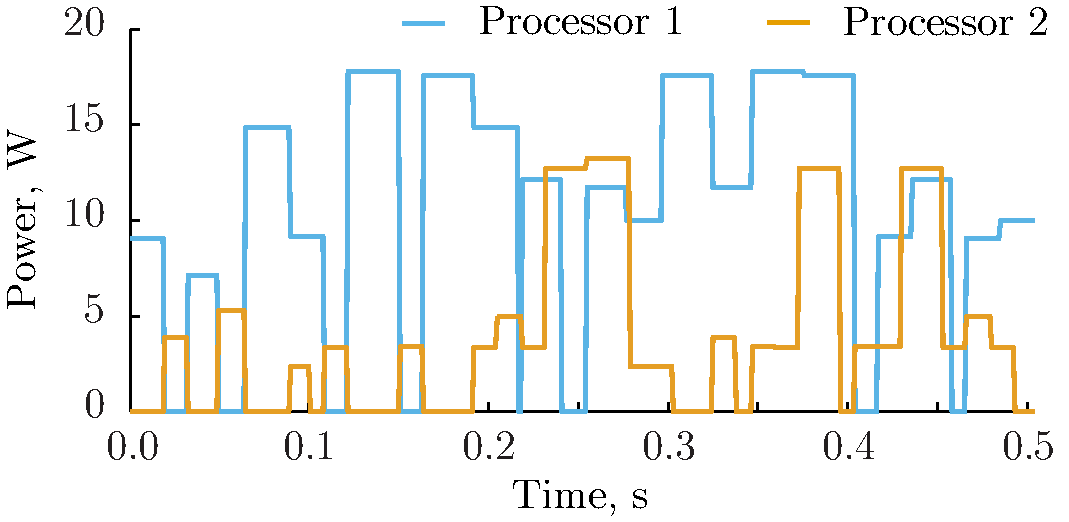
\includegraphics[width=1.00\columnwidth]{include/assets/application-power.pdf}
  \vspace{-0.5em}
  \caption{A dynamic power profile.}
  \flabel{application-power}
  \vspace{-0.5em}
\end{figure}

Assume that the dynamic power profile, $\profilePdyn$, corresponding to the considered workload is the one shown in \fref{application-power}.

\begin{figure}[bl]
  \vspace{-1.0em}
  \centering
  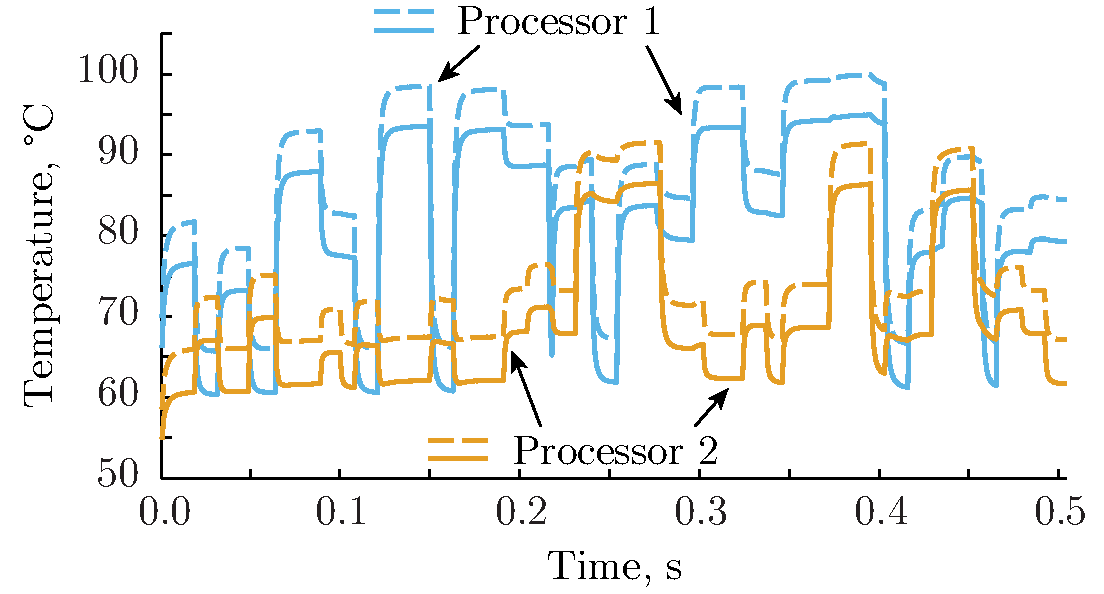
\includegraphics[width=0.90\columnwidth]{include/assets/application-temperature.pdf}
  \vspace{-0.5em}
  \caption{The expected temperature (the solid lines) and one standard deviation above it (the dashed lines).}
  \flabel{application-temperature}
\end{figure}

The expansion for power has the same structure but different coefficients.
Such a series might be shorter or longer depending on the accuracy requirements.
As we see, our surrogate model has a negligibly small computational cost to undertake UQ at \stage{5}: for any outcome of the uncertain parameters $\vZ(\o) \equiv \vZ$, we can easily compute the corresponding temperature by plugging $\vZ$ into the above equation; the same applies for power.
Thus, such characteristics as \cdfs\ and \pdfs\ (see \fref{motivation-pdf}) can be rigorously estimated. Furthermore, the expectation and variance at the $k$th moment of time are calculated as simply as
\[
  \oExp{\vTO_k(\o)} = \pccs_{k1} \hspace{1em} \text{and} \hspace{1em} \oVar{\vTO_k(\o)} = \sum_{i = 2}^{6} \pcn_i \: \pccs_{ki}^2
\]
where $\pcn_i$ are normalization constants, and the squaring should be understood element-wise.
For the nominal power profile $\profilePdyn$ depicted in \fref{application-power}, we obtain the corresponding stochastic temperature profile $\profileT{\o}$ and can observe, \eg, its expectation and standard deviation; they are plotted in \fref{application-temperature}.
The displayed curves closely match those obtained via MC simulations with $10^4$ samples; however, our method takes less than a second, on a personal laptop, while MC sampling takes more than a day, which we discuss in \sref{experimental-results}.


\subsection{Post-processing} \slabel{output-processing}
Due to the properties of PC expansions, specifically, due to the basis functions and their pairwise orthogonality (see \aref{orthogonal-polynomials}), the obtained polynomial traces are trivial for various prospective analyses. For instance, consider the PC expansion of temperature at the $k$th time interval given as
\begin{equation} \elabel{pc-k}
  \oPC{\vars}{\pcorder}{\vTO_k(\o)} = \sum_{i = 1}^{\pcterms} \pcc{\vTO}_{ki} \pcb_i(\vZ(\o))
\end{equation}
where $\pcc{\vTO}_{ki}$ are computed using \eref{fourier-output} and \eref{pc-recurrence}. Let us, for example, find the expectation and variance of the expansion. As shown in \aref{spectral-projection}, these statistics have the following simple expressions solely based on the coefficients:
\begin{equation} \elabel{pc-moments}
  \oExp{\vTO_k(\o)} = \pcc{\vTO}_{k1} \hspace{1em} \text{and} \hspace{1em} \oVar{\vTO_k(\o)} = \sum_{i = 2}^{\pcterms} \pcn_i \: \pcc{\vTO}_{ki}^2
\end{equation}
for expectation and variance, respectively, where the squaring is element-wise, and $\pcn_i$ are normalization constants. Furthermore, global and local sensitivity analyses of deterministic and non-deterministic quantities can be readily conducted on \eref{pc-k}; see, \eg, \cite{eldred2009, maitre2010}. The \cdf\ as well as the \pdf\ can be estimated by sampling \eref{pc-k}. Each sample is a trivial evaluation of a polynomial; on the contrary, when a MC-based technique is employed to perform UQ of \eref{fourier-system}, a sample is a complete simulation of $\profPdyn$. Since the number of such samples should be considerably large, \eg, in the order of $10^4$ \cite{xiu2010, diaz-emparanza2002}, to obtain reliable results, MC-based approaches become highly time-consuming and often infeasible for practical applications.

